% !TeX root = RJwrapper.tex
\title{Stats: An R Package for Statistics}
\author{by Shylock and Antonio}

\maketitle

\abstract{%
An abstract of less than 150 words.
}

\hypertarget{introduction}{%
\section{Introduction}\label{introduction}}

This paper will highlight how modern day Shylock would love to use the
\CRANpkg{stats} for his actuarial and money lending interests . The same
could be applicable for Antonio for managing his risk properly had he
analyzed and predicted his ship routes and data well.

\hypertarget{background}{%
\section{Background}\label{background}}

I use the stats package a lot for my actuarial and general interest in
data science. Hence this package is a daily driver for me. The various
functions such as arima and acf help me in estimation and modelling of
time series data.

\begin{figure}
\centering
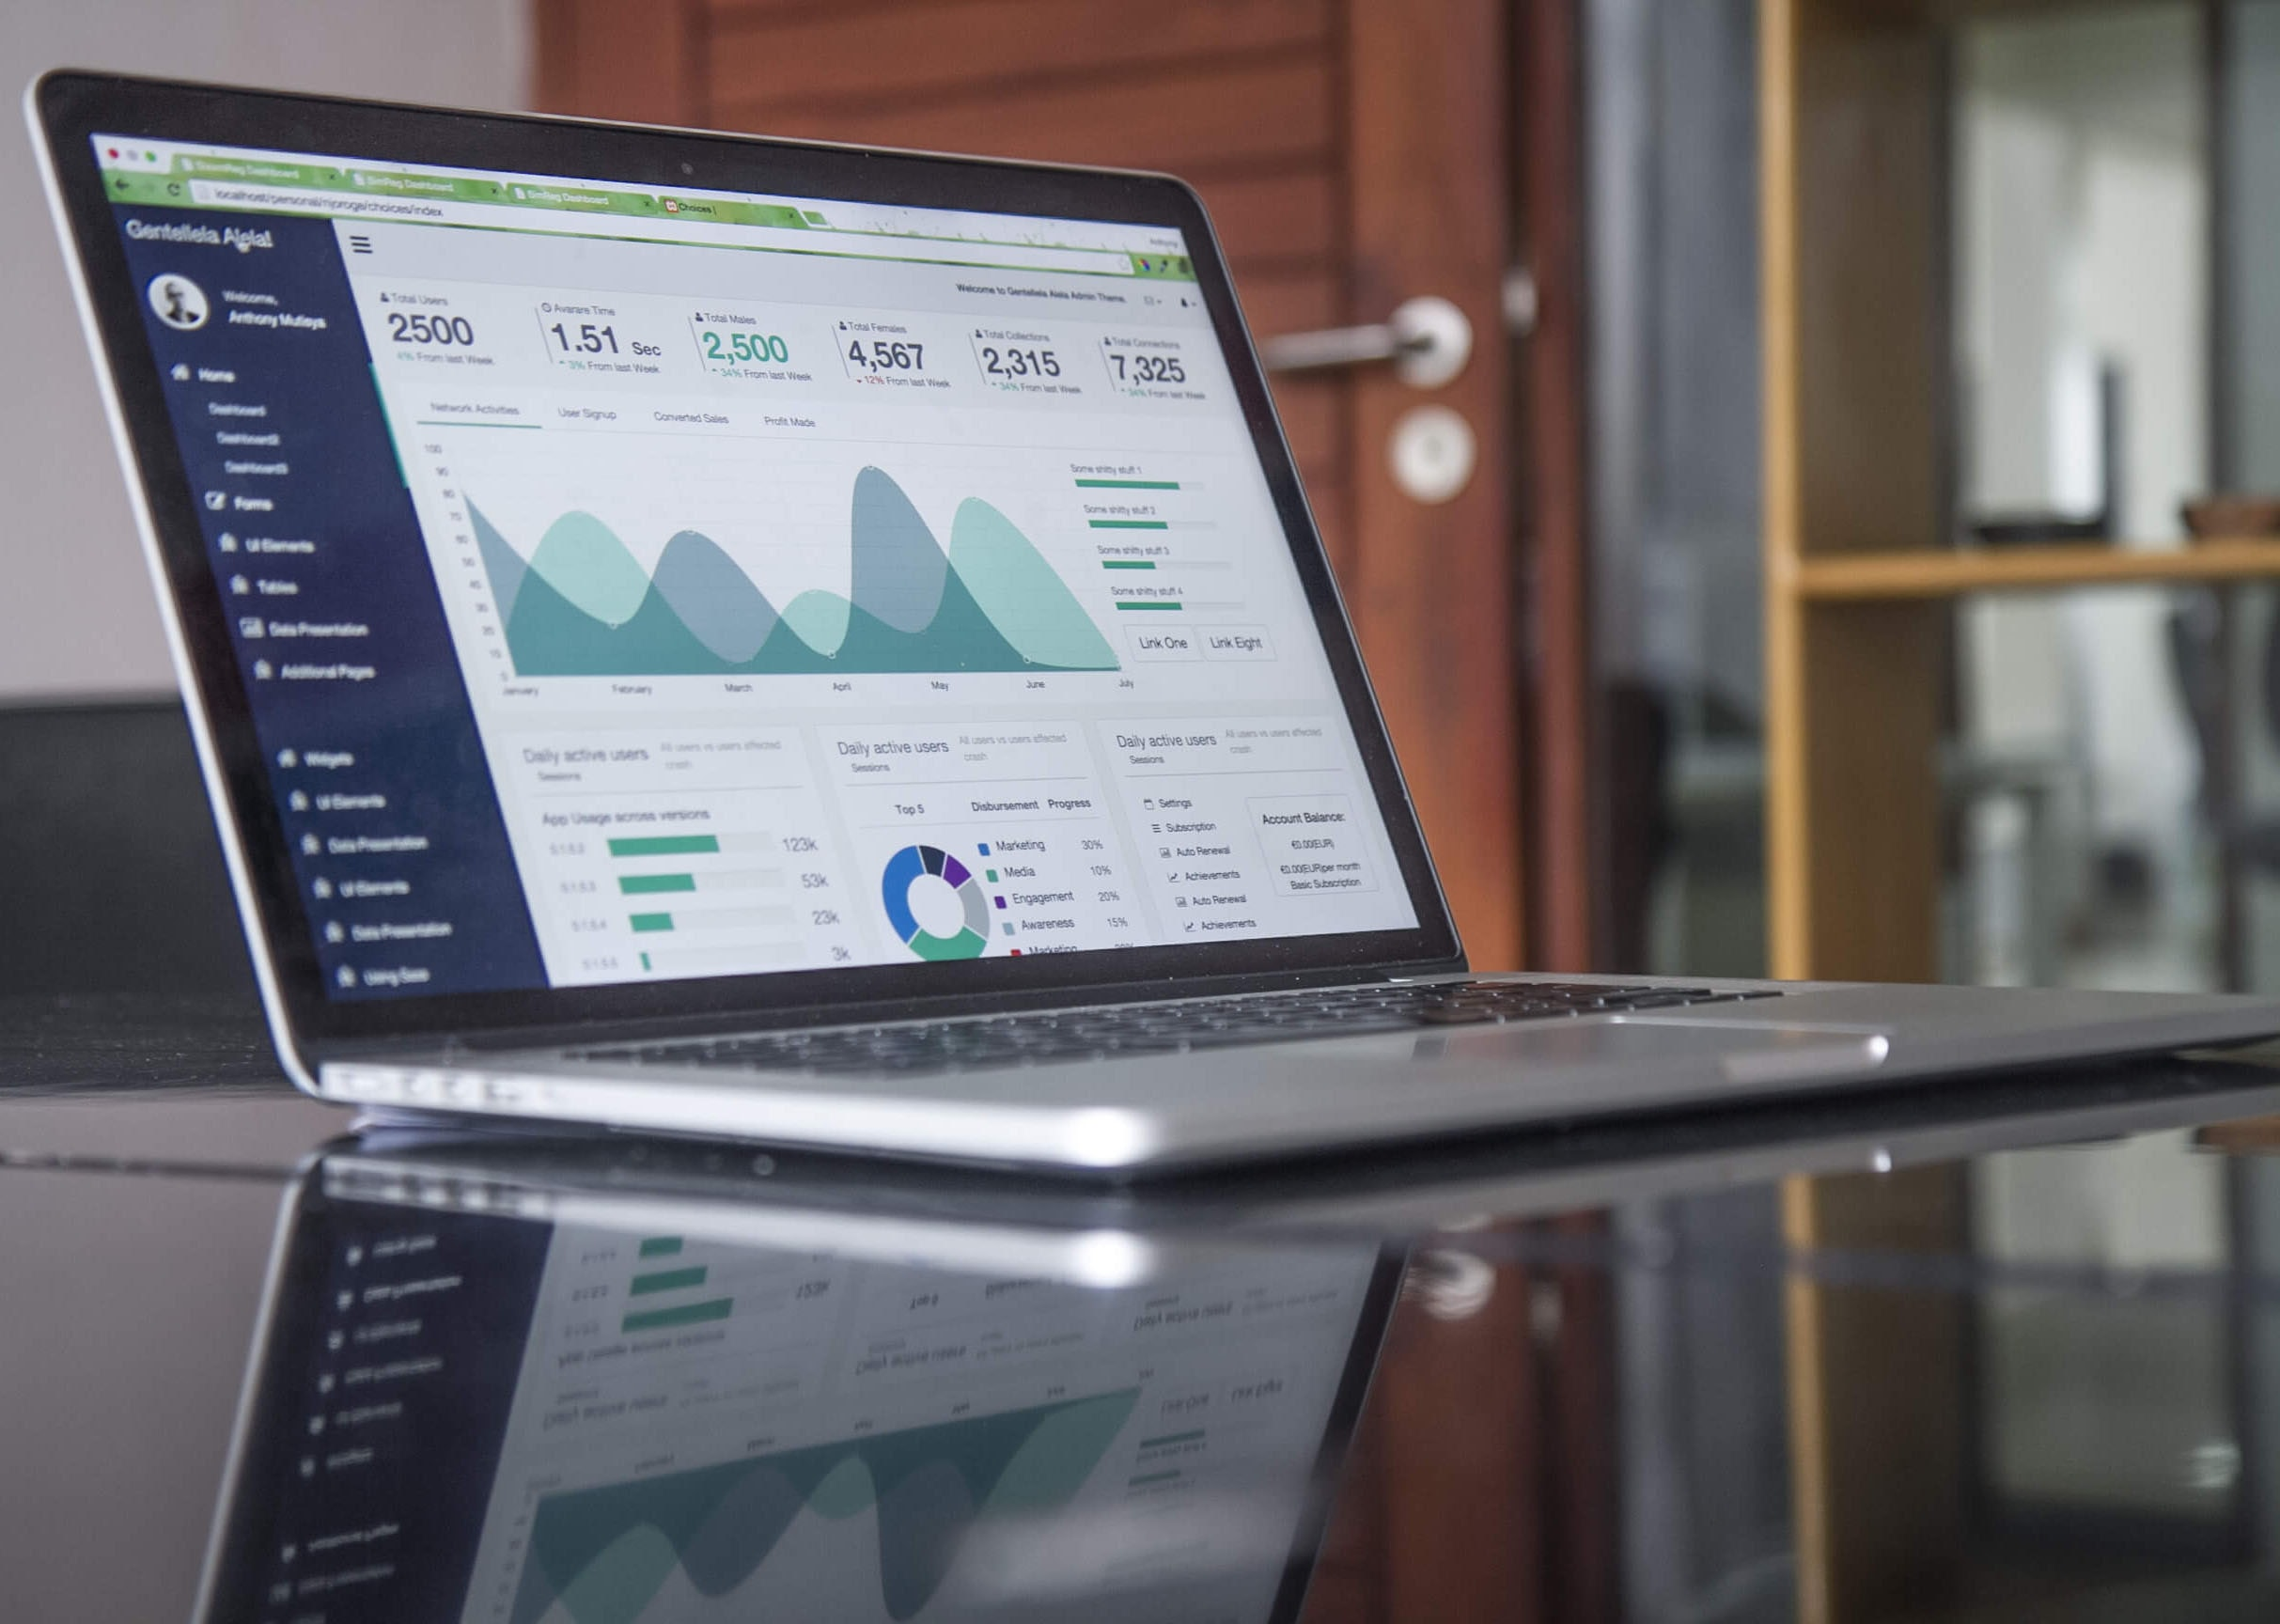
\includegraphics[width=0.6\textwidth,height=2.60417in]{stat.jpg}
\caption{A possible stat dashboard}
\end{figure}

\hypertarget{a-gallery-of-stats-examples}{%
\section{A gallery of stats
examples}\label{a-gallery-of-stats-examples}}

\hypertarget{the-autocovariance-of-the-log-of-airpassengers-data-using-the-acf-function.}{%
\subsection{1. The AutoCovariance of the log of AirPassengers data using
the acf
function.}\label{the-autocovariance-of-the-log-of-airpassengers-data-using-the-acf-function.}}

\begin{Schunk}

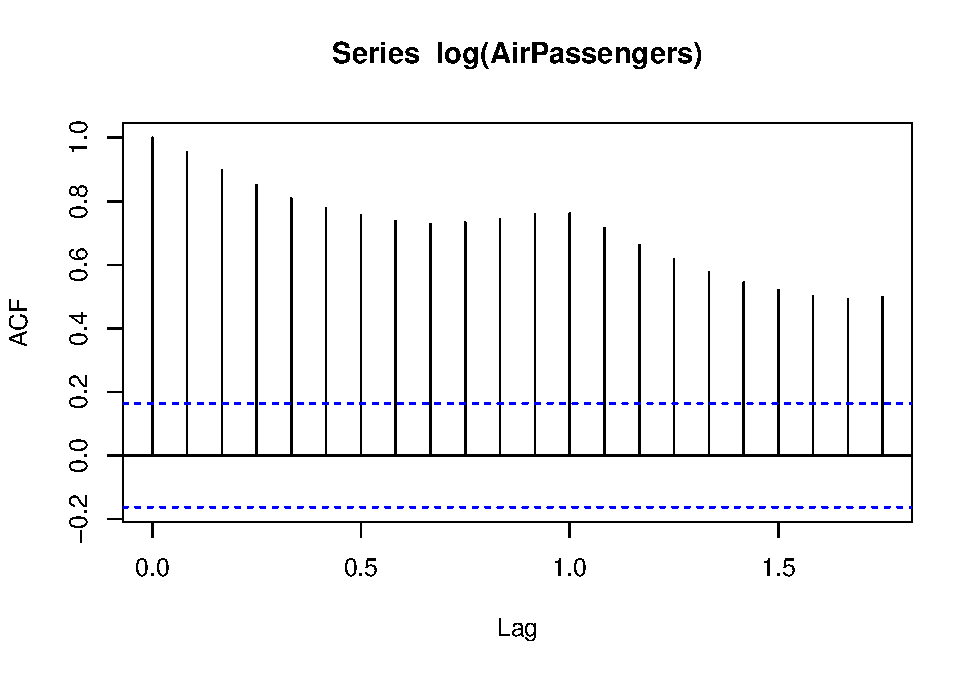
\includegraphics{Abhi-1U_files/figure-latex/unnamed-chunk-1-1} \end{Schunk}

\hypertarget{creating-a-arima-model-for-air-passengers}{%
\subsection{2. Creating a ARIMA model for Air
Passengers}\label{creating-a-arima-model-for-air-passengers}}

\begin{Schunk}
\begin{Soutput}
#> 
#> Call:
#> arima(x = log(AirPassengers), order = c(0, 1, 1), seasonal = list(order = c(0, 
#>     1, 1), period = 12))
#> 
#> Coefficients:
#>           ma1     sma1
#>       -0.4018  -0.5569
#> s.e.   0.0896   0.0731
#> 
#> sigma^2 estimated as 0.001348:  log likelihood = 244.7,  aic = -483.4
\end{Soutput}
\end{Schunk}

\hypertarget{summary}{%
\section{Summary}\label{summary}}

We have demonstrated some Stat functions that are available in the
package \pkg{stats}.

\bibliography{RJreferences.bib}

\address{%
Shylock\\
Money-Lender\\%
Somewhere in Venice\\ Italy\\
%
%
\textit{ORCiD: \href{https://orcid.org/0000-1721-1511-1101}{0000-1721-1511-1101}}\\%
\href{mailto:shylock@money.com}{\nolinkurl{shylock@money.com}}%
}

\address{%
Antonio\\
Trader\\%
The Docks\\ Somewhere in Venice, Italy\\
%
\url{https://www.britannica.com/animal/bilby}\\%
\textit{ORCiD: \href{https://orcid.org/0000-0002-0912-0244}{0000-0002-0912-0244}}\\%
\href{mailto:antonio@trader.com}{\nolinkurl{antonio@trader.com}}%
}
